\documentclass[9pt]{beamer}
\usepackage[english, russian]{babel}
\usepackage[T2A]{fontenc}
\usepackage[utf8]{inputenc}
\usepackage{indentfirst}
\usepackage{amsmath, amsfonts, amssymb, amsthm, mathtools}
\usepackage[export]{adjustbox}
\usepackage{graphicx} 
\graphicspath{ {./images/} }

\usepackage{subcaption}
\usepackage{verbatim}

\usepackage{hyperref}

\hypersetup{
    colorlinks=true,
    linkcolor=blue,
    filecolor=magenta,      
    urlcolor=black,
    pdftitle={Overleaf Example},
    pdfpagemode=FullScreen,
    }

% \usepackage[table]{xcolor}
% \usepackage{array}
\usepackage{multirow}
\usepackage{colortbl}

\title{Лабораторная работа № 2. \\ Расчёт сети Fast Ethernet}
\author{Данила Стариков \\ НПИбд-02-22}
\institute{Российский университет дружбы народов имени Патриса Лумумбы}
\date{\today}

\begin{document}

\frame{\titlepage}

\begin{frame}
\frametitle{Цель работы}
\begin{itemize}
    \item Оценить работоспособность 100-мегабитной сети Fast Ethernet в соответствии
    с первой и второй моделями.
\end{itemize}
\end{frame}

\begin{frame}
\frametitle{Топология сети}
    \centering
        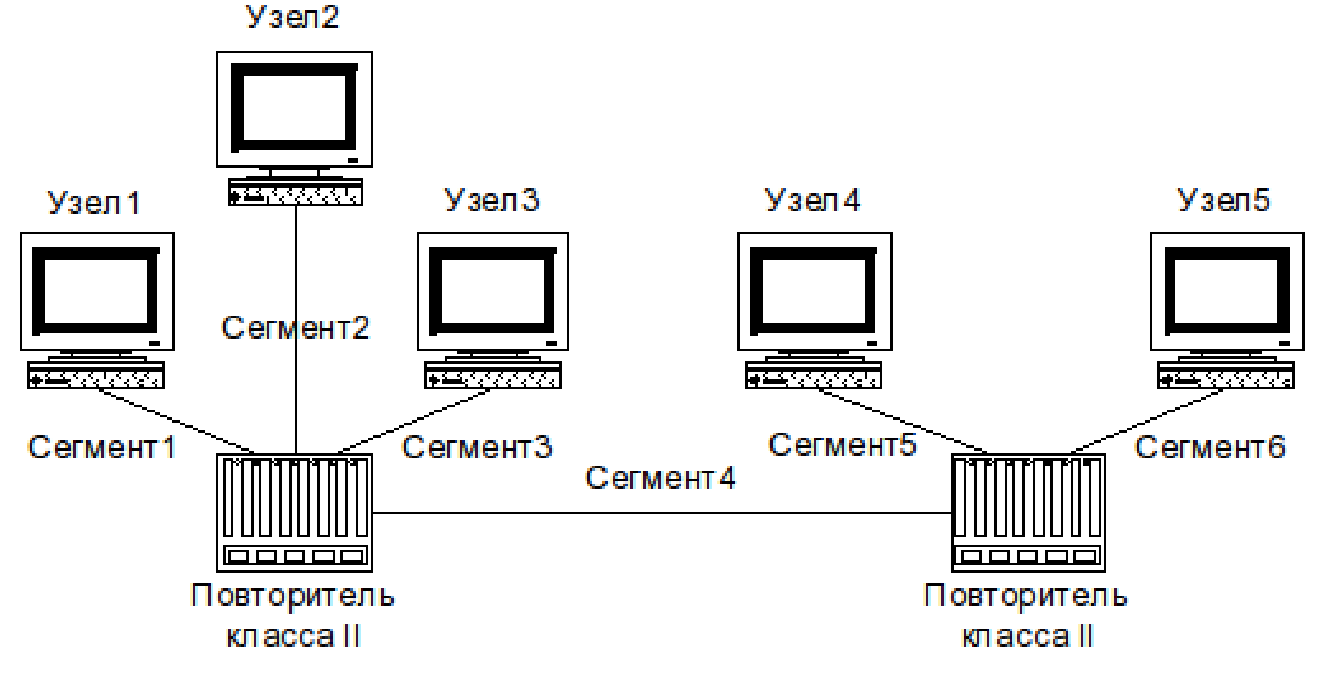
\includegraphics[width=\textwidth]{../images/topology.png}
\end{frame}

\begin{frame}
\frametitle{Конфигурации сети}
    \begin{tabular}{|c|c|c|c|c|c|c|}
    \hline
        Вариант & Сег-т 1 & Сег-т 2 & Сег-т 3 & Сег-т 4 & Сег-т 5 & Сег-т 6 \\ \hline
        1 & 96 & 92 & 80 & 5 & 97 & 97 \\ \hline
        2 & 95 & 85 & 85 & 90 & 90 & 98 \\ \hline
        3 & 60 & 95 & 10 & 5 & 90 & 100 \\ \hline
        4 & 70 & 65 & 10 & 4 & 90 & 80 \\ \hline
        5 & 60 & 95 & 10 & 15 & 90 & 100 \\ \hline
        6 & 70 & 98 & 10 & 9 & 70 & 100 \\ \hline
    \end{tabular}
\end{frame}

\begin{frame}
\frametitle{Первая модель}
\begin{tabular}{|c|c|c|c|c|c|c|m{1cm}|}
    \hline
    Вар. & Сег-т 1 & Сег-т 2 & Сег-т 3 &\cellcolor{lightgray} Сег-т 4 & Сег-т 5 & Сег-т 6 & Диаметр домена коллизий \\ \hline
        1 &\cellcolor{orange} 96 & 92 & 80 &\cellcolor{orange} 5 &\cellcolor{orange} 97 & 97 & 198 \\ \hline
        2 &\cellcolor{orange} 95 & 85 & 85 &\cellcolor{orange} 90 & 90 &\cellcolor{orange} 98 & \cellcolor{red} 283 \\ \hline
        3 & 60 &\cellcolor{orange} 95 & 10 &\cellcolor{orange} 5 & 90 &\cellcolor{orange} 100 & 200 \\ \hline
        4 &\cellcolor{orange} 70 & 65 & 10 &\cellcolor{orange} 4 &\cellcolor{orange} 90 & 80 & 164 \\ \hline
        5 & 60 &\cellcolor{orange} 95 & 10 &\cellcolor{orange} 15 & 90 &\cellcolor{orange} 100 &\cellcolor{red} 209 \\ \hline
        6 & 70 &\cellcolor{orange} 98 & 10 &\cellcolor{orange} 9 & 70 &\cellcolor{orange} 100 &\cellcolor{red} 207 \\ \hline
    \end{tabular}
\colorbox{orange}{Оранжевый фон} - Сегмент принадлежит домену коллизий.
\colorbox{red}{Красный фон} - Вариант конфигурации сети не работоспособен.
\end{frame}

\begin{frame}
\frametitle{Вторая модель}
\begin{table}[!ht]
    \caption{Временные задержки компонентов сети}
    \label{tab:data}
    \centering
    \begin{tabular}{|m{5cm}|l|}
    \hline
        Компонент пути & Время двойного оборота, би \\ \hline
        Пара терминалов с интерфейсами TX & 100 \\ \hline
        Сегмент на витой паре категории 5 (на 1 метр) & 1.112 \\ \hline
        Повторитель класса II  & 92 \\ \hline
    \end{tabular}
\end{table}
\end{frame}

\begin{frame}
\frametitle{Вторая модель}
\begin{tabular}{|m{2.5cm}|l|l|l|l|l|l|}
    \hline
    \multirow{3}{*}{Компонент пути} & \multicolumn{6}{|c|}{Время двойного оборота, би} \\ \cline{2-7}
                                    & \multicolumn{6}{|c|}{Вариант} \\ \cline{2-7}
                                    & 1 & 2 & 3 & 4 & 5 & 6 \\ \hline
        Пара терминалов с интерфейсами TX & 100 & 100 & 100 & 100 & 100 & 100 \\ \hline
        Первый сегмент на витой паре & 106.7 & 105.6 & 105.6 & 77.9 & 105.6 & 109.0 \\ \hline
        Второй сегмент на витой паре & 5.56 & 100.1 & 5.6 & 4.4 & 16.7 & 10.0 \\ \hline
        Третий сегмент на витой паре & 107.9 & 109.0 & 111.2 & 100.1 & 111.2 & 111.2 \\ \hline
        Повторитель класса II & 92 & 92 & 92 & 92 & 92 & 92 \\ \hline
        Повторитель класса II & 92 & 92 & 92 & 92 & 92 & 92 \\ \hline
        Врема двойного оборота сети, би & 504.176 & \cellcolor{red} 598.7 & 506.4 & 466.4 &\cellcolor{red} 517.5 &\cellcolor{red} 514.2 \\ \hline
    \end{tabular}
\colorbox{red}{Красный фон} - Вариант конфигурации сети не работоспособен.
\end{frame}
\begin{frame}
\frametitle{Выводы}
\begin{itemize}
    \item В рамках лабораторной работы изучили принципы технологии Ethernet и Fast Ethernet
и на практике познакомились с методиками оценки работоспособности сети, построенной
на базе технологии Fast Ethernet.
\end{itemize}
\end{frame}
\end{document}
